\documentclass{article}
\usepackage{graphicx}
\usepackage[margin=1.5cm]{geometry}
\usepackage{amsmath}
\usepackage{hyperref}

\begin{document}

\title{Week 3 Writing Activity: \textit{Hierarchy of Detail}}
\author{Prof. Jordan C. Hanson (INTD100)}

\maketitle

\textbf{Video Solution for This Exercise}: \url{https://youtu.be/g1q_6JDNpdg}
\begin{figure}
\centering
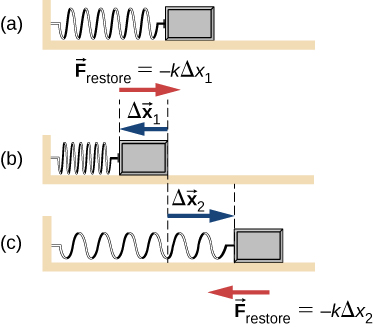
\includegraphics[width=0.33\textwidth]{figures/spring.jpeg}
\caption{\label{fig:1} A spring exerts a force on a mass when compressed or stretched.}
\end{figure}

\section{Concise Writing I: Hierarchy of Detail Exercise}

Consider the following paragraph, describing an experiment we perform to measure the strength of a spring (see Fig. \ref{fig:1}).
\begin{quotation}
Let \textbf{F} be the force of the spring, \textit{k} be the constant of proportionality between force and displacement, and \textbf{x} be the displacement.  The force of a spring is proportional to the distance it is displaced from its equilibrium length.  The force is always in the opposite direction as the displacement.  According to Hooke's Law, $\mathbf{F} = -k\mathbf{x}$.  The force applied to the spring, given the total mass \textit{M} hung from it, will be \textit{M} times the gravitational constant, \textit{g}.  Each displacement \textit{x} may be recorded alongside \textit{Mg}, so that $k$ will be $Mg/\mathbf{x}$.  To measure the k-value of a spring, we may hang weights of known masses from the spring, while recording the new length as each weight is added.
\end{quotation}

Reorganize the sentences above so that they are in the proper hierarchy of detail.  The new paragraph should make more sense.
\end{document}
